%% -*- LaTeX -*- This is LaTeX2e code
\documentclass{elsart}
%\usepackage{fullpage}
\usepackage{algorithmic}
\usepackage{algorithm}
\usepackage{graphicx}
\journal{CGTA}

\newcommand{\Oh}[1]{\ensuremath{\mathcal{O}(#1)}}
\newcommand{\Wm}[1]{\ensuremath{\Omega(#1)}}
\newcommand{\orderof}[1]{\ensuremath{\Theta(#1)}}
%\newcommand{\etal}{\emph{et~al.}}
\newcommand{\ournote}[1]{\marginpar{#1}}
\newtheorem{lemma}{Lemma}
\newtheorem{theorem}{Theorem}
\newcommand{\text}[1]{\textrm{#1}}
\setlength{\parskip}{1em}

\newcommand{\floor}[1]{\left\lfloor #1 \right\rfloor}
\newcommand{\ceil}[1]{\left\lceil #1 \right\rceil}

\newcommand{\patscomment}[1]{}


%\ifdraft
%\date{Draft as of \today}
%\fi

\begin{document}
\begin{frontmatter}
\title{Space-Efficient Geometric Divide-and-Conquer
Algorithms\thanksref{funding}}
\thanks[funding]{This research was supported in part by grants from
NSERC and DAAD grant D/0104616.}
\author[carleton]{Prosenjit Bose}
\author[carleton]{Anil Maheshwari}
\author[carleton]{Pat Morin}
\author[carleton]{Jason Morrison}
\author[carleton]{Michiel Smid}
\author[muenster]{Jan Vahrenhold}
\address[carleton]{School of Computer Science, Carleton University, 
         1125 Colonel By Drive, \\ Ottawa, Ontario, Canada, K1S~5B6}
\address[muenster]{Westf\"{a}lische Wilhelms-Universit\"{a}t,
    Institut f\"{u}r Informatik, 48149 M\"{u}nster, Germany} 

\begin{abstract}
  We develop a number of space-efficient tools including an approach
  to simulate divide-and-conquer space-efficiently, stably selecting
  and unselecting a subset from a sorted set, and computing the $k$th
  smallest element in one dimension from a multi-dimensional set that
  is sorted in another dimension.  We then apply these tools to solve
  several geometric problems that have solutions using some form of
  divide-and-conquer. Specifically, we present a deterministic
  algorithm running in $\Oh{n \log n}$ time using $\Oh{1}$ extra
  memory given inputs of size $n$ for the closest pair problem and a
  randomized solution running in $\Oh{n \log n}$ expected time and
  using $\Oh{1}$ extra space for the bichromatic closest pair problem.
  For the orthogonal line segment intersection problem, we solve the
  problem in $\Oh{n\log n + k}$ time using $\Oh{1}$ extra space where
  $n$ is the number of horizontal and vertical line segments and $k$
  is the number of intersections.
\end{abstract}
\end{frontmatter}

\section{Introduction}

Researchers have studied space-efficient algorithms since the early
1970's. Examples include merging, (multiset) sorting, and partitioning
problems; see, for example,
references~\cite{geffert:merging,katajainen:partitioning,katajainen:multisets}.
Br\"onnimann \etal~\cite{bronnimann:convex} were the first to consider
space-efficient geometric algorithms and showed how to compute the
convex hull of a planar set of $n$ points in \Oh{n \log h} time using
\Oh{1} extra space, where $h$ denotes the size of the output (the
number of extreme points).  Recently, Chen and
Chan~\cite{chen:space-efficient} addressed the problem of computing
all the intersections among a set of $n$ line segments, giving an
algorithm that runs in \Oh{(n+k)\log^2 n} time using \Oh{\log^2n}
extra space where $k$ is the number of intersections and an algorithm
that runs in \Oh{(n+k)\log n} time using \Oh{1} extra space but the
initial input is destroyed.  Br\"onnimann, Chan, and
Chen~\cite{bronnimann:inplace} developed some space efficient data
structures and used them to solve a number of geometric problems such
as 3-dimensional convex hull, Delaunay triangulation and nearest
neighbour queries.  Br\"onnimann and Chan \cite{bronnimann:melkman}
describe $\Oh{1}$ extra-memory algorithms for computing the convex
hull of simple (open or closed) polygonal chains. 

In this paper, we develop a number of space-efficient tools outlined
in Section \ref{sec:tools} that are of interest in their own right. We
then apply these tools to several geometric problems that have
solutions using some form of divide-and-conquer. Specifically, we
address the problems of closest pairs, bichromatic closest pairs and
orthogonal line segment intersection.

\subsection{The Model}

The goal is to design algorithms that use very little extra space over
and above the space used for the input to the algorithm. The input is
assumed to be stored in an array of size $n$, thereby allowing random
access.  The specifics of the input are outlined with each problem
addressed.  We assume that a constant size memory can hold a constant
number of words. Each word can hold one pointer, or an \Oh{\log n} bit
integer, and a constant number of words can hold one element of the
input array. The extra memory used by an algorithm is measured in
terms of the number of extra words. In certain cases, the output may
be much larger than the size of the input. For example, given a set of
$n$ line segments, if the goal is to output all the intersections,
there may be as many as \Wm{n^2}. In such cases, we consider the
output memory to be write-only space usable for output but cannot be
used as extra storage space by the algorithm.  This model has been
used by Chen and Chan~\cite{chen:space-efficient} for variable size
output, space-efficient algorithms and accurately models algorithms
that have output streams with write-only buffer space. Equivalently
the algorithm could report the output one item at a time by calling
some user-defined subroutine for each item.

The remainder of the paper is organized as follows. In Section
\ref{sec:tools}, we outline the space-efficient tools that will be
useful in the solution of the geometric problems addressed. In Section
\ref{sec:nn}, we present an \Oh{n \log n} time algorithm to solve the
closest pair problem using only \Oh{1} extra memory. In the following
subsection, we solve the bichromatic closest pair problem in \Oh{n
\log n} expected time using only \Oh{1} extra memory. The solution is
randomized but the extra memory used is still \Oh{1} in the worst
case.  Section \ref{sec:orth} presents a solution to the orthogonal
line segment intersection problem in \Oh{n\log n + k} time using
\Oh{\log n} extra space where $n$ is the number of line segments, and
$k$ is the number of intersections.  Conclusions and open problems are
in Section \ref{sec:conc}.  The details of an \Oh{1} extra memory
algorithm for orthogonal line segment intersection appear in
Appendix~\ref{sec:olsi}.


%\begin{definition}
%  An algorithm that needs \Oh{1} extra working space is called
%  \emph{in-place}, and an algorithm that needs \Oh{\log_2 n} extra
%  space is called \emph{in situ}.
%\end{definition}
%
%Recently, Raman~\etal~\cite{raman:dynamic,raman:indexable} considered 
%\emph{succinct} representations of ordered sets that allowed for
%various dictionary operations.
%
%%% Local Variables:
%%% mode: latex
%%% TeX-master: "paper"
%%% End:


%% -*- LaTeX -*- This is LaTeX2e code

\section{Space-Efficient Tools} \label{sec:tools}

In this section, we outline a number of algorithmic tools that will be
useful in the sequel.  We begin with a general scheme for implementing
divide-and-conquer algorithms and then present tools for selecting
subsets and finding the element of a given rank without disturbing the
input array.

\subsection{Space-Efficient Divide-and-Conquer}\label{sec:dc}

In this subsection, we describe a simple scheme for space-efficiently
performing divide-and-conquer. In a standard recursive procedure,
prior to each recursive call, the current state of the procedure (i.e.
the state of the variables, program counter, etc.)  that is invoking
the recursive call is saved on a stack.  The variables making up the
current state are often referred to as the {\em activation frame} and
the stack is usually called the {\em recursion stack}. 
%According to
%our model, a constant amount of memory is sufficient to store one
%activation frame on the recursion stack. 
Thus, in the standard
recursive approach, the amount of extra space needed for the recursion
stack is directly proportional to the height of the recursion tree
times the
number of local variables.

A template for recursive divide-and-conquer algorithms that partition
into 2 subproblems of equal size is presented as
Algorithm~\ref{alg:template} (\textsc{Recursive}). It operates on an
array $A[0,\ldots,n-1]$.  The algorithm makes calls to 4 subroutines:
\textsc{Base-Code} is used to solve small instances, \textsc{Pre-Code}
is executed before any recursive calls, \textsc{Mid-Code} is executed
after the first recursive call but before the second, and
\textsc{Post-Code} is executed after the second recursive call.
Normally, the functions \textsc{Pre-Code} and \textsc{Post-Code}
perform the divide step and the conquer step, respectively.  If the
functions \textsc{Pre-Code}, \textsc{Mid-Code} and \textsc{Post-Code}
all run in $\Oh{e-b}$ time then the total running time of a call to
$\textsc{Recursive}(A,0,n)$ is \Oh{n\log n}.

\begin{algorithm}
  \caption{$\textsc{Recursive}(A,b,e)$: Standard template recursive
    divide-and-conquer}
  \label{alg:recurse}
  \label{alg:template}
  \begin{algorithmic}[1]
    \IF{$e-b \le 2^{h_0}$ where $s$ is the size of the recursion base.}
    \STATE $\textsc{Base-Code}(A,b,e)$ 
           \COMMENT{Code for solving small instances}
    \ELSE
    \STATE $\textsc{Pre-Code}(A,b,e)$ 
           \COMMENT{Computations to setup Subproblem 1 in 
                    $A[b,\ldots,\lfloor e/2 \rfloor-1]$}
    \STATE $\textsc{Recursive}(A,b,\lfloor e/2 \rfloor)$ 
           \COMMENT{First recursive call}
    \STATE $\textsc{Mid-Code}(A,b,e)$ \COMMENT{Computations to setup Subproblem 2 in
            $A[\lfloor e/2\rfloor,\ldots,e-1]$}
    \STATE $\textsc{Recursive}(A,\lfloor e/2 \rfloor,e)$
           \COMMENT{Second recursive call}
    \STATE $\textsc{Post-Code}(A,b,e)$ 
       \COMMENT{Computations to merge Subproblems 1 and 2 in
       $A[b,\ldots,e-1]$}
    \ENDIF
  \end{algorithmic}
\end{algorithm}

To develop in-place divide-and-conquer algorithms, we must do two
things:  (1)~We must use a stack of size $\Oh{1}$ and (2)~we must
implement the functions $\textsc{Pre-Code}$, $\textsc{Mid-Code}$ and
$\textsc{Post-Code}$ using only $\Oh{1}$ extra space.  Note that, if we
use Algorithm~\ref{alg:template} directly then the stack space
required is $\Omega(\log n)$ since the recursion tree has depth
$\Theta(\log n)$.  In the remainder of this section we show how this
stack space can be reduced to $\Oh{1}$.

The main idea is to perform a stackless traversal of the binary
recursion tree.  Algorithms for stackless traversals of trees date
back at least to Knuth \cite[Section~2.3.2]{knuth:fundamental}.  The
algorithm for traversing a binary tree without a stack is quite
simple;  it maintains a pointer to the current node $u$ and a state
$s$ that keeps track of whether the algorithm has already visited 0
(pre), 1 (mid) or 2 (post) of $u$'s children.  Using four simple rules,
the algorithm then decides whether the next node visited will be the
parent, the left child of $u$, or the right child of $u$ and also
decides on the next state.

\newcommand{\pre}{\mathrm{pre}}
\newcommand{\midd}{\mathrm{mid}}
\newcommand{\post}{\mathrm{post}}

\begin{algorithm}
\begin{algorithmic}[1]
\caption{$\textsc{Stackless-Recursive}(A)$: Stackless simulation
of $\textsc{Recursive}(A,0,n)$} \label{alg:stackless}
\STATE{$u\gets 0$ \COMMENT{The current node}}
\STATE{$h\gets \log_2 n$ \COMMENT{The height of the current node}}
\STATE{$s\gets\pre$ \COMMENT{The current state}}
\WHILE{$h \le \log_2 n$}
  \IF{$h=h_0$ \COMMENT{$u$ is a leaf}}
    \STATE{$\textsc{Base-Code}(A,u,u+2^h)$}
    \STATE{\COMMENT{Next we visit the parent of $u$}}
    \STATE{$s\gets\mbox{$\midd$ or $\post$}$ (depending on whether
$u_h$ is 0 or 1, respectively)}
    \STATE{$u_h\gets 0$}
    \STATE{$h\gets h+1$}
  \ELSIF{$s = \pre$}
    \STATE{$\textsc{Pre-Code}(A,u,u+2^h)$}
    \STATE{\COMMENT{Next we visit left child of $u$}}
    \STATE{$s\gets \pre$}
    \STATE{$h\gets h-1$} 
    \STATE{$u_h\gets 0$}
  \ELSIF{$s = \midd$}
    \STATE{$\textsc{Mid-Code}(A,u,u+2^h)$}
    \STATE{\COMMENT{Next we visit right child of $u$}}
    \STATE{$s\gets \pre$}
    \STATE{$h\gets h-1$}
    \STATE{$u_h\gets 1$}
   \ELSIF{$s = \post$}
    \STATE{$\textsc{Post-Code}(A,u,u+2^h)$}
    \STATE{\COMMENT{Next we visit parent of $u$}}
    \STATE{$s\gets\mbox{$\midd$ or $\post$}$ (depending on whether
$u_h$ is 0 or 1, respectively)}
    \STATE{$u_h=0$}
    \STATE{$h\gets h+1$}
  \ENDIF
\ENDWHILE
\end{algorithmic}
\end{algorithm}

In our case, the binary tree we are traversing is implicit.  For
simplicity, we assume that $n$ is a power of 2, so that all leaves of
the recursion tree are at the same level.  The algorithm, which is
described by the pseudocode given in Algorithm~\ref{alg:stackless} uses a
$\lceil\log_2 n\rceil$-bit integer $u$ to keep track of the path from
the root to the current node.  Here, and throughout, we use the
notation $u_h$ to denote the $h$th most significant bit of $u$.  (This
bit represents $2^h$.) The integer $u$ represents the path as a sequence
of 0's and 1's (0 for a left turn and 1 for a right turn).  The
algorithm also maintains an integer $h$ to keep track of the height
(distance to the leaves) of $u$.  In this way, the length of the path
from $u$ to the root of the tree is $\log_2 n - h$.  With this
representation the pair $(u,h)$ represents a subproblem of size $2^h$
that begins at position $u$, i.e., the subarray $A[u,\ldots,u+2^h-1]$.
It is an easy exercise \cite[Exercise~10.4-5]{cormen:alg} to see that if $n$ is a power of 2
then Algorithm~\ref{alg:stackless} performs exactly the same calls to
$\textsc{Base-Code}$, $\textsc{Pre-Code}$, $\textsc{Mid-Code}$, and
$\textsc{Post-Code}$, and in the same order as
Algorithm~\ref{alg:template}. Furthermore, this transformation does not
increase the overall running time by more than an additive linear term.

\begin{theorem}\label{thm:stackless}
For $n$ a power of two, Algorithm~\ref{alg:stackless} performs the same
computations as Algorithm~\ref{alg:template} using only $\Oh{1}$ extra
space beyond what is used by the functions \textsc{Base-Code},
\textsc{Pre-Code}, \textsc{Mid-Code}, and \textsc{Post-Code}.
Furthermore, if the running time of Algorithm~\ref{alg:template} is
$T(n)$ then the running time of Algorithm~\ref{alg:stackless} is
$T(n)+\Oh{n}$.
\end{theorem}

\noindent\textbf{Remark:}  Theorem~\ref{thm:stackless} only addresses
the case when $n$ is a power of 2. The general case can be handled by
traversing the recursion tree for a problem of size $2^{\lceil\log_2
n\rceil}$ and simply adding checks to Algorithm~\ref{alg:stackless} to
make sure that it does not access any non-existent array elements.

We now have the first ingredient required for \Oh{1} extra-memory
recursive algorithms: a constant-size simulation of the recursion
stack.  In the next few sections, we develop some tools that help with
the second ingredient required for in-place divide-and-conquer
algorithms.  In particular, these tools help to implement the
functions \textsc{Pre-Code}, \textsc{Mid-Code} and \textsc{Post-Code}
using $\Oh{1}$ extra space.

\patscomment{
In most divide-and-conquer situations, the recursion tree is balanced,
implying that only $\Oh{\log n}$ extra space is needed for maintaining
the recursion stack when the input has size $n$.  In randomized
algorithms, such as Quicksort, the recursion tree can have linear
height in the worst case. However, by always recursing on the smaller
sub-array first\footnote{This is sometimes referred to as optimizing
tail recursion.}, a worst case size of $\Oh{\log n}$ for the stack can
be maintained\cite{huang:one-way,wegner:generalized}.  Consider
Algorithm \ref{alg:recurse} below, which represents a generic template
for divide-and-conquer algorithms.  Note that ``PROCESS x" simply
refers to a set of non-recursive statements.


Can a balanced recursion tree arising from the above recursive
algorithm be traversed with only $\Oh{1}$ extra memory as opposed to the
$\Oh{\log n}$ extra memory used for the stack?  Our technique outlines a
method for converting any algorithm fitting the above recursive
template into one that uses only $\Oh{1}$ extra memory. The recursion
tree is traversed in the same manner without use of the recursion
stack. In many cases, the same type of result can be obtained using
bottom-up merge, however, it is well known that bottom-up merge has
poor performance in the presence of caches.

The main idea (which is probably folklore, even though we have not
seen it explicitly in the literature) is to simulate a post-order
traversal of the recursion tree. We assume for simplicity that the
data to be processed is stored in an array $A=A[0,\ldots,n-1]$ of size
$n = 2^k$ for some positive integer $k$. The recursion tree
corresponding to the above divide-and-conquer scheme is a perfectly
balanced binary tree, in which each node at depth $0 \leq i < k$
corresponds to a subarray of the form $A[j \cdot 2^{k-i} ,\ldots, (j +
1) \cdot 2^{k-i} - 1]$ for some integer $0 \leq j \leq i$.\footnote{If
the problem size is not an exact power of two, we imagine the
recursion tree to be embedded into a perfectly balanced tree and stop
traversing the tree prematurely.}

Our scheme is presented in Algorithm~\ref{alg:traversal}. We maintain
two indices $b$ and $e$ that indicate the subarray $A[b ,\ldots, e-1]$
currently processed. We will use the binary representation of the
index $e$ to implicitly store the current status of the post-order
traversal, i.e., the node of the simulated recursion tree currently
visited.

\begin{algorithm}
  \caption{$\textsc{Stackless-Recursive}(b,e)$: Stackless simulation
of \textsc{Recursive}}
  \label{alg:traversal}
  \begin{algorithmic}[1]
    \STATE $b=0$ and $e=s$, $s$ is the size of the recursion base.
    \WHILE{$b\neq 0$ or $e\leq n$}
    \STATE \{PROCESS 1: Base instance operations. Process all items in
$A[b,\ldots, e-1]$.\}
    \STATE $i$ be the index of the least significant bit of $e$.
    \FOR{$c\gets 1,\ldots, i$}
    \STATE $b \gets e-2^c$.
    \STATE \{PROCESS 3: Pre-merge operations\}
    \STATE Merge  $A[b,\ldots, b+2^{c-1} - 1]$ with
$A[b+2^{c-1},\ldots, e-1]$
    \STATE \{PROCESS 4: Post-merge operations on $A[b,\ldots, e-1]$ \}
    \ENDFOR 
    %\STATE $b \gets e$.  Not needed because of line 7.
    \STATE $e \gets e + s$.
    \ENDWHILE
  \end{algorithmic}
\end{algorithm}

Determining the value of $i$ (Step 4) can be done in $\Oh{1}$ amortized
time without extra space using a straightforward implementation of a
binary counter.  The above algorithm basically traverses the recursion
tree from left to right. When processing a leaf $v$, the algorithm
backtracks in geometrically increasing steps merging all subtrees
already traversed completely. This merging is done by traversing a
leaf-to-root path starting from $v$ but stopping as soon as the path
goes up to the right (Figure~\ref{fig:tree_spaceefficient}). The
correctness of the algorithm follows from the next
lemma\cite{cormen:alg}:

\begin{lemma}
  If the leaves of a complete binary tree are labeled from left to
  right (starting with $1$ for the leftmost leaf), the height of the
  largest subtree containing the leaf $e>1$ as its rightmost leaf is
  equal to the index $i$ of the least significant bit of the number
  $e$.
\end{lemma}

\begin{figure}
  \centerline{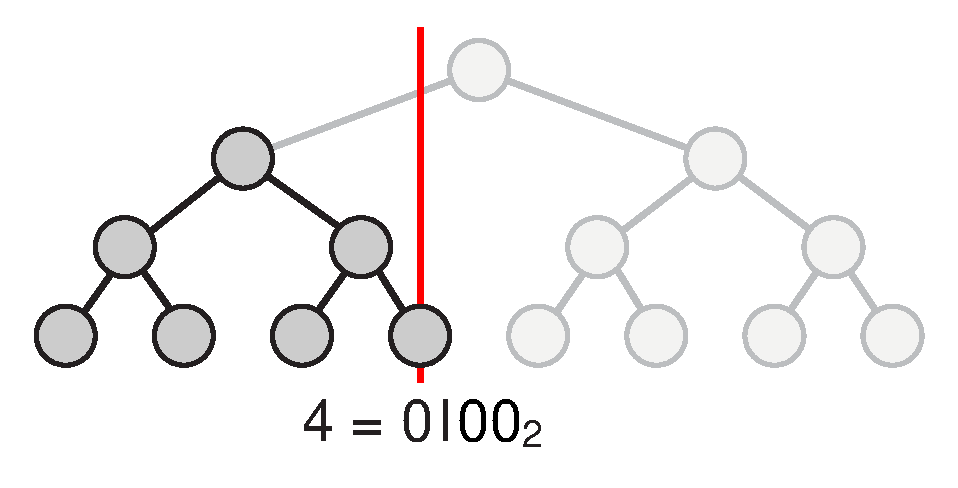
\includegraphics[height=3.5cm]{tree_spaceefficient}}
  \caption{Merging subtrees while traversing left-to-right.}
  \label{fig:tree_spaceefficient}
\end{figure}

Therefore, any algorithm that is in the form outlined by Algorithm
\ref{alg:recurse} using $\Oh{\log n}$ extra space can be transformed
into a space-efficient algorithm of the form Algorithm \ref{alg:traversal}
using only $\Oh{1}$ extra space provided that all the base instances
(i.e. leaves of the recursion tree) can be pre-computed with only \Oh{1} extra
space and PROCESS 1,3,4 as well as the Merge step can be made
space efficient using only \Oh{1} extra space. Note that PROCESS 2
operations no longer need to be computed in Algorithm \ref{alg:traversal}
since we assume that the array is initially partitioned into the
base instances. Therefore, there is no need to actually partition
the array as is done in PROCESS 2 in Algorithm \ref{alg:recurse}. Henceforth, we will refer
to recursive algorithms in standard form (i.e. Algorithm
\ref{alg:recurse}) as the {\em standard recursive form} and
space-efficient recursive algorithms (i.e. Algorithm \ref{alg:traversal})
as {\em space-efficient recursive form}. We conclude this section
with the following:



\begin{theorem}
An algorithm in standard recursive form running in \Oh{n \log n} time and using \Oh{\log n} extra space can be converted
to space-efficient recursive form running in \Oh{n \log n} time using only \Oh{1} extra space provided that all the base instances
(i.e. leaves of the recursion tree) can be pre-computed in \Oh{n \log n} time with only \Oh{1} extra
space and PROCESS 1,3,4 as well as the Merge step can be made
space efficient using only \Oh{1} extra space and \Oh{n} time.
\end{theorem}

Note that there can be trade-offs in the above theorem. For example, if in the space-efficient recursive form, the Merge step takes
\Oh{n \log n} time then, the overall running time becomes \Oh{n \log^2 n}. These trade-offs are fairly straightforward, related to the
Master Theorem for Recurrences \cite{cormen:alg} and can be adjusted to each situation.

}


\subsection{Sorted Subset Selection}

In this subsection, we introduce a simple yet surprisingly powerful
algorithm, called \textsc{SubsetSelection}.
%%$(A,b,e,f)$. 
The algorithm provides a way of selecting a subset of the elements and
moving them to the front of the array without changing their relative
order.  What makes this algorithm so powerful is that, if the array is
initially sorted according to some total order $<$ then it is possible
(in fact very easy) to undo the effects of the algorithm to restore
the original sorted order.  We note that stable partitioning
algorithms and stable merging algorithms could achieve the same
effect, but these algorithms are an order of magnitude more
complicated than the code given here.

The \textsc{SubsetSelection} algorithm, given in pseudocode as
Algorithm~\ref{alg:sortedSubsetSelection}, stably moves to the front
of the array all elements in $A[b,\ldots, e-1]$ for which the given
$(0,1)$-valued selection function $f$ returns the value 1.

\begin{algorithm}
  \caption{Algorithm
    $\textsc{SubsetSelection}(A,b,e,f)$ for selecting a
    subset from a sorted array $A[b,\ldots, e-1]$.} 
  \label{alg:sortedSubsetSelection}\label{alg:subsetselection}
  \begin{algorithmic}[1]
    \REQUIRE Array $A[b,\ldots, e-1]$ is sorted and $f$ is a 
    $(0,1)$-valued function that can be evaluated in constant
    time.
    
    \ENSURE $A[b,\ldots, m-1]$ contains all entries for which
    $f$ is one, and these entries are still sorted.

    \STATE $i\gets b$, $j\gets b$ and $m\gets b+1$. 
    \WHILE{$i<e$ \textbf{and} $j<e$}
      \WHILE{$i<e$ \textbf{and} $f(A[i])=1$}
        \STATE $i\gets i+1$. \COMMENT{Move index $i$ such that
          $f(A[i])=0$.} 
      \ENDWHILE
      \STATE $j\gets i+1$;
      \WHILE{$j<e$ \textbf{and} $f(A[j])=0$}
        \STATE $j\gets j+1$. \COMMENT{Move index $j$ such that
        $f(A[j])=1$.} 
      \ENDWHILE
      \IF{$j<e$}
        \STATE \textbf{swap} $A[i]\leftrightarrow A[j]$.
        %\STATE $m\gets i+1$. \COMMENT{$A[b,\ldots, m-1]$
        %  contains all 1-valued entries.}
      \ENDIF
    \ENDWHILE
    \STATE Return $i$.
  \end{algorithmic}
\end{algorithm}

Algorithm~\ref{alg:sortedSubsetSelection} clearly uses only \Oh{1}
extra space and runs in linear time. The correctness of the algorithm
follows from the loop invariant that is maintained: $A[b,\ldots, i-1]$
stably contains all selected elements from $A[b,\ldots, e-1]$ whose rank
is at most $i-b$.  The effects of this algorithm can be reversed by
Algorithm~\ref{alg:revertSubsetSelection}.

\begin{algorithm}
  \caption{Algorithm $\textsc{UndoSubsetSelection}(A,b,e,i)$
    for restoring the total order after applying the 
    \textsc{SubsetSelection}-Algorithm~\ref{alg:sortedSubsetSelection}}
  \label{alg:revertSubsetSelection}\label{alg:undosubsetselection}
  \begin{algorithmic}[1]

    \REQUIRE{Array $A[b,\ldots, e-1]$ contains the result of running
      Algorithm~\ref{alg:sortedSubsetSelection} on array
      $A[b,\ldots, e-1]$ that was sorted} 
    \ENSURE{Array $A[b,\ldots, e-1]$ is sorted}
    
    \STATE $i\gets i-1$ and $j\gets e-1$
    \WHILE{$i\neq j$ and $i\geq b$}
      \IF{$A[j]<A[i]$}
        \STATE \textbf{swap} $A[i]\leftrightarrow A[j]$
        \STATE $j\gets j-1$
      \ENDIF
      \STATE $i\gets i-1$
    \ENDWHILE

  \end{algorithmic}
\end{algorithm}

There is one important property to note:
Algorithm~\ref{alg:revertSubsetSelection} does not require knowledge
of the selection function $f$, but only needs to know the three
indices $b$, $e$ and $i$. It uses only comparisons to recover the
state prior to the invocation of \textsc{SubsetSelection}. This is a
key property that is useful particularly if the selection function $f$
is unknown or cannot be easily reconstructed.  In the following
subsection, we show how useful \textsc{SubsetSelection} and its
counterpart \textsc{UndoSubsetSelection} are.


\subsection{Selecting the $k$-th smallest element}\label{sec:sel}

In designing in-place geometric algorithms, the ability to undo
operations such as selection turns out to be extremely useful.  In
this section, we show how we can select the $k$th smallest element
according to some total order $<_x$ in an array that is sorted
according to some other total order $<_y$.  Once the $k$th smallest
element is found, the original ($<_y$) sorted order of the array is
restored.  Our algorithm is a modification of Hoare's \textsc{Find}
algorithm \cite{hoare:find}.

The original \textsc{Find} algorithm selects a random pivot and
partitions the array $A$ into the subset of elements that are less
than or equal to the pivot and the subset of elements that are greater
than the pivot and then searches recursively in one of these two
parts.  The partitioning and undoing of the partitioning can be
accomplished using Algorithms~\ref{alg:subsetselection} and
\ref{alg:undosubsetselection}.  However, for
Algorithm~\ref{alg:undosubsetselection} to work it needs to know the
sizes of each of the two parts of the array (remembering the pivot
element also works).  Unfortunately, remembering these sizes for each
recursive invocation of the algorithm produces a stack of expected
size $\Theta(\log n)$.  To get around this problem, we force the
algorithm to always partition the current array into two parts of size
\emph{exactly} $\floor{3n/4}$ and $\ceil{n/4}$.

This idea is implemented as Algorithm~\ref{alg:selectk}
(\textsc{Select}).  Suppose without loss of generality that $k\le
n/2$.  Then we find an element $p$ whose rank is between $n/2$ and
$3n/4$.  Since there are at least $\floor{n/4}$ such elements, with
only an expected constant number of random selections, we can find
such an element.  Computing the rank of a given element takes \Oh{n}
time, thus in \Oh{n} expected time, we can find $p$. Note that if we
partition the array with $p$, then at least $n/4$ elements can be
eliminated.  The key is to eliminate {\em precisely} $n/4$ elements.
This way, when it comes time to undo the operation, we know exactly
where the partition boundaries occur. This is where the stack $S$
comes into play.  Each time through the loop, we reduce the size of
the array to $\lfloor 3n/4 \rfloor$. To undo this operation, we need
to record the actual remainder from the division by $3/4$. Two bits
are sufficient to record this since the remainder can only be one of
$\{0, 1, 2, 3\}$.  For example, suppose that the current instance has
an array of size 37.  Since $3\times 37/4 = 27+3/4$, the next instance
has size $27$ and we push the remainder $3$ on the stack.  In the undo
step, if the current instance is of size 27, to recover the size of
the array at invocation, we note that $(4\times 27 + 3)/3 = 37$ which
is the computation used to recover the indices required for the Undo
operation.


\begin{algorithm}
  \caption{Algorithm
    $\textsc{Select}(A,0,e,k)$ Select the $k$th smallest element in
    $A[0,\ldots,e-1]$ according to the total order $<_x$.}

  \label{alg:selectk}\label{alg:find}
  \begin{algorithmic}[1]
    \REQUIRE Array $A[0,\ldots, e-1]$ is sorted according to $<_y$
    \ENSURE The $k$-th smallest element according to $<_x$ is placed at
$A[0]$, and $A[1,\ldots, e-1]$ is sorted by $<_y$

    \STATE $n \gets e$. \COMMENT{$n$ is the current size of the array being processed.}
    \WHILE{$n > 42$}
          \IF{$k < n/2$}
             \STATE Pick a random element $p$ whose rank is between $n/2$ and $3n/4$
             \STATE Use \textsc{SubsetSelection} to move all elements
$<_x p$ and a sufficient number $>_x p$ to fill $A[0,\ldots,\lfloor 3n/4 \rfloor - 1]$
             \STATE Push $4(3n/4 - \lfloor 3n/4 \rfloor)$ on stack $S$
             \STATE $n \gets \lfloor 3n/4 \rfloor$
          \ELSE
             \STATE Pick a random element $p$ whose rank is between $n/4$ and $n/2$
             \STATE Use \textsc{SubsetSelection} to move all elements
$>_x p$ and a sufficient number $<_x p$ to fill $A[0,\ldots,\lfloor 3n/4 \rfloor - 1]$
             \STATE Push $4(3n/4 - \lfloor 3n/4 \rfloor)$ on stack $S$
             \STATE $k \gets k - \lceil n/4 \rceil$
             \STATE $n \gets \lfloor 3n/4 \rfloor$
          \ENDIF
    \ENDWHILE
    \STATE Find $k$-th smallest element $q$ in $A[0,\ldots,n-1]$ by brute force
    \STATE $M \gets n$
    \STATE $R \gets \mathrm{pop}(S)$
    \STATE $D \gets (4M + R)/3$
    \WHILE{$D < e$}
          \STATE UndoSubsetSelection($A,0,D,M$)
          \STATE $M \gets D$.
          \STATE $R \gets \mathrm{pop}(S)$
          \STATE $D \gets (4M + R)/3$
    \ENDWHILE
    \STATE Find $q$ in $A[0,\ldots, e-1]$ and move it stably to $A[0]$
  \end{algorithmic}
\end{algorithm}

In the final loop where the steps are {\em undone}, the only
information we require are the three indices $0, D$ and $M$. We do not
need to remember the particular element $p$ that was used in the
\textsc{SubsetSelection} step.  Comparisons of $Y$-coordinates
are sufficient to recover the original order. 

Since at each iteration through the while loop, we eliminate a quarter
of the elements, the number of iterations through the loop is \Oh{\log
n}. At each iteration, two bits are pushed on the stack, so the total
number of bits ever stored in the stack is \Oh{\log n} which implies
that only \Oh{1} extra space is used. The running time of the
algorithm is given by the following recurrence: \[ T(n) = T(3n/4) +
\Oh{n} \] which resolves to \Oh{n}.

This algorithm can be made to run in \Oh{n} deterministic time. The
only step where randomization is used is in the selection of the
partition element $p$. In the deterministic version, we use techniques
from the algorithm by Blum \etal~\cite{blum:selection}.  Instead of
selecting an element at random, we select the partition element by
first decomposing the array into $n/5$ groups of 5 elements and
computing the median of the medians of the groups.  The idea is simple
and similar to the above algorithm except some of the details are
quite tedious, so we outline the details in Appendix
\ref{sec:detkmed}.

\section{Closest Pair Problems}\label{sec:nn}

\subsection{Closest Pair}

Given a set $P$ of $n$ points in the plane stored in an array
$A[0,\ldots,n - 1]$, a closest pair is a pair of points in
$P$ whose Euclidean distance is smallest among all pairs of points. We
modify an algorithm by Bentley and
Shamos~\cite{bentley:divide-and-conquer} to compute the closest pair
in \Oh{n \log n} time using only \Oh{1} extra space.

Algorithm~\ref{alg:bentley} gives pseudocode for a slightly modified
version of the Bentley-Shamos divide-and-conquer algorithm for finding
the closest pair.  The algorithm works by drawing an imaginary
vertical dividing line through the median $X$-coordinate.  The
algorithm then finds the closest pair with both points to the left of
this line, the closest pair with both points to the right of this line
and then finds the closest pair with one point on the left and one
point on the right of the line.  The first two closest pairs are
computed with recursive calls while the third closest pair is
accomplished by a vertical plane sweep of all the points that are
``close to'' the dividing line.  Details of this plane sweep can be
found in the original paper \cite{bentley:divide-and-conquer}.
 
\begin{algorithm} \label{alg:nn}
  \caption{$\textsc{Closest-Pair}(A,b,e)$: Divide-and-Conquer algorithm for finding a closest
    pair~\cite{bentley:divide-and-conquer}.}\label{alg:bentley} 
  \begin{algorithmic}[1]
    \REQUIRE All points in the input array $A$ are sorted according to
    $Y$-coordinate.
    \ENSURE The first two points in the array $A[b,\ldots,e-1]$ realize the closest pair and the remaining points are sorted by $Y$-coordinate.
    \IF{$e-b < 16$} 
      \STATE Compute a closest pair using a brute-force
algorithm, stably place them at $A[b]$ and $A[b+1]$.
    \ELSE
      \STATE Compute the median $X$-coordinate $x$ of $A[b,\ldots,e-1]$ using
Algorithm~\ref{alg:selectk} (\textsc{Select}) while maintaining the array
sorted by $Y$-coordinate.
      \STATE Using Algorithm~\ref{alg:sortedSubsetSelection}
(\textsc{SubsetSelection}), stably select all
elements of $A[b,\ldots,e-1]$ with $X$-coordinate less than or equal $x$ so
that they are stored in $A[b,\ldots,\lfloor e/2\rfloor-1]$. 
      \STATE $\textsc{Closest-Pair}(A,b,\lfloor e/2 \rfloor)$
      \STATE Using Algorithm~\ref{alg:revertSubsetSelection}
(\textsc{UndoSubsetSelection}), restore
$A[b,\ldots,e-1]$ so that it is sorted by $Y$-coordinate.  Stably store the
closest pair from the previous step in $A[b]$ and $A[b+1]$.
       \STATE Using Algorithm~\ref{alg:sortedSubsetSelection}
(\textsc{SubsetSelection}), stably select all elements of $A[b,\ldots,e-1]$ with $X$-coordinate greater than $x$ so that they are stored in
$A[\lfloor e/2\rfloor,\ldots,e-1]$. 
      \STATE $\textsc{Closest-Pair}(A,\lfloor e/2 \rfloor,e)$
       \STATE Using Algorithm~\ref{alg:revertSubsetSelection}
(\textsc{UndoSubsetSelection}), restore
$A[b,\ldots,e-1]$ so that it is sorted by $Y$-coordinate.  Stably store the
closest pair from Step~6 or the closest pair from the previous step (whichever
is closer) at
locations $A[b]$ and $A[b+1]$.
      \STATE Let $\delta$ be the distance between $A[b]$ and $A[b+1]$.
      \STATE Using Algorithm~\ref{alg:sortedSubsetSelection}
(\textsc{SubsetSelection}), extract in $Y$-sorted order the points of $A[b,\ldots,e-1]$ that fall within a
                strip of width $2\delta$ centered at the median $X$-coordinate of $A[b,\ldots,e-1]$.
         \STATE Scan the points in this strip to determine whether it
contains a pair of
                points with distance smaller than $\delta$. Update $\delta$ and
                the closest pair as necessary. 
        \STATE Using Algorithm~\ref{alg:revertSubsetSelection}
(\textsc{UndoSubsetSelection}), restore
$A[b,\ldots,e-1]$ so that it is sorted by $Y$-coordinate.  Stably store the closest pair 
at
locations $A[b]$ and $A[b+1]$.
    \ENDIF
  \end{algorithmic}
\end{algorithm}


Note that if we let the work done in Line~2 be denoted by
\textsc{Base-Code}, the work done in Lines~4 and 5 be denoted by
\textsc{Pre-Code}, the work in Lines~7 and 8 denoted by
\textsc{Mid-Code} and the work done in Lines~10--14 by
\textsc{Post-Code} then the algorithm is identical to
Algorithm~\ref{alg:template}.  Furthermore, all of these routines use
only $\Oh{1}$ extra space. Therefore, by Theorem~\ref{thm:stackless},
the entire algorithm can be implemented using only $\Oh{1}$ extra space.

\begin{theorem}
  Given a set $P$ of $n$ points in the plane stored in an array
  $A[0, \ldots, n-1]$, a closest pair in $P$ can be computed in
  \Oh{n \log n} time using \Oh{1} extra memory.
\end{theorem}


\subsection{Bichromatic Closest Pair}

In the Bichromatic Closest Pair Problem, we are given a set $R$ of red
points and a set $B$ of blue points in the plane. The problem is to
return a pair of points, one red and one blue, whose distance is
minimum over all red-blue pairs. We assume that there are a total of
$n=r+b$ points, with $r>0$ red points and $b>0$ blue points.  The
input is given to us as two arrays $R[0,\ldots,r-1]$ and
$B[0,\ldots,b-1]$. 
 
The algorithm we use, which to the best of our knowledge is new, is
similar to the Bentley-Shamos algorithm from the previous section, but
has some subtle differences.  The algorithm chooses a vertical line,
computes the closest bichromatic pair to the left of the line, the
closest bichromatic pair to the right of the line and the closest
bichromatic pair with one point on the left of the line and one point
on the right of the line.  The difficulties arise in two places.  The
first is that, in general there does not exist a vertical line that
partitions each of $R$ and $B$ into two sets of equal size.  If we
choose a line that partitions $R$ into two equal sets then we obtain
an uneven partition of $B$ and vice-versa.  The second difficulty is
that, in order to obtain a running time of \Oh{n\log n}, we need a
linear time algorithm for finding the closest pair between two sets
separated by a line.  We concentrate first on the second problem.

\subsubsection{Computing the closest vertically separated pair}

In this subsection we give pseudocode in Algorithm~\ref{alg:separated}
(\textsc{Bichromatic-Closest-Vertically-Separated-Pair}) for computing
the closest bichromatic pair separated by a given vertical line
$\ell$.  We concentrate on the case in which $R$ and $B$ are separated
by $\ell$ with $R$ to the left of $\ell$ and $B$ to the right of
$\ell$.  It is clear that if we can solve this case then we can solve
the general case using two calls to this algorithm and a constant
number of calls to $\textsc{SubsetSelection}$ and
$\textsc{UndoSubsetSelection}$.

\begin{algorithm}
  \caption{\textsc{Bichromatic-Closest-Vertically-Separated-Pair}($R,B,\ell$): Bichromatic closest pair when $R$ and $B$ are separated by
    a vertical line $\ell$ and $R$ is to the left of $\ell$.} 
  \label{alg:bichromatic-separated}\label{alg:separated}
  \begin{algorithmic}[1]
    \REQUIRE All points in $R[0,\ldots,r-1]$ and $B[0,\ldots,b-1]$ are sorted by
    $Y$-coordinate 
    \ENSURE All points in $R$ and $B$ are sorted by
    $Y$-coordinate, and the bichromatic closest pair is reported
    \STATE $r\gets |R|$ and $b\gets |B|$.
    \WHILE{$r> 16$ and $b>16$}
        \STATE Assume $r\geq b$, otherwise reverse the roles of $R$ and $B$
        \REPEAT
        \STATE Pick a random element $p$ from $R[0,\ldots,r-1]$
        \STATE Find the distance $\delta$ from $p$ to the nearest
    element of $B[0,\ldots,b-1]$
        \STATE Compute the left envelope of disks having radius
               $\delta$ centered at each of the points in $B[0,\ldots,b-1]$.
        \UNTIL{at least $\floor{r/2}$ elements of $R[0,\ldots,r-1]$ are to the
left of the envelope}
               \STATE Move exactly $\lfloor r/2\rfloor$ elements from
$R[0,\ldots,r-1]$ that are not to the left of the blue 
                      envelope into $R[0,\lfloor r/2 \rfloor -1]$. 
               \STATE Push $2(r/2 - \lfloor r/2 \rfloor)$ on the stack $S$.
               \STATE Push 1 bit on stack $S$ when $r \geq b$ and 0 bit otherwise.
               \STATE Undo the envelope computation.
               \STATE $r \gets \lfloor r/2 \rfloor$.
    \ENDWHILE
    \STATE Compute and report a bichromatic closest pair using a
    brute-force algorithm since one of $r$ of $b$ is at most 16
    \STATE\COMMENT{Undo operations to restore $Y$-sorted order for
both $R$ and $B$}
    \WHILE {$r < |R|$ or $b < |B|$}
         \STATE $F \gets \mathrm{pop}(S)$
         \STATE $X \gets \mathrm{pop}(S)$
         \IF{$F$ is 1 (i.e. $r \geq b$)}
            \STATE $r_1 \gets 2r + X$ 
            \STATE $\textsc{UndoSubsetSelection}(R,0,r_1,r)$.
            \STATE $r \gets r_1$.
         \ELSE 
            \STATE \COMMENT{$F$ is 0 (i.e. $r < b$)}
            \STATE $b_1 \gets 2b + X$.
            \STATE $\textsc{UndoSubsetSelection}(B,0,b_1,b)$.
            \STATE $b \gets b_1$.
         \ENDIF
    \ENDWHILE
  \end{algorithmic}
\end{algorithm}

\begin{figure}
  \centerline{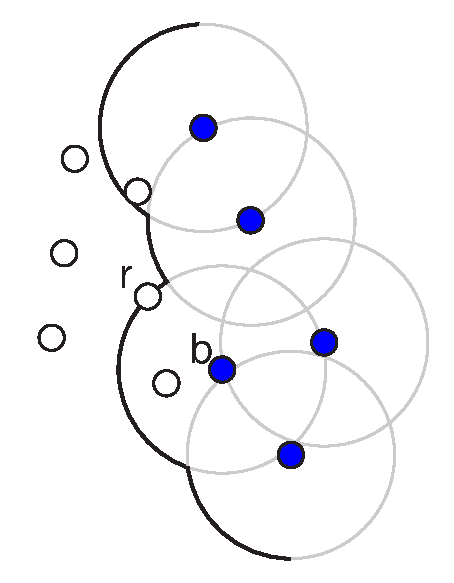
\includegraphics[height=5cm]{biclosest_algorithm}}
  \caption{Left envelope of disks centered at blue points (red
    points are drawn as hollow disks).}
  \label{fig:biclosest_algorithm}
  \label{fig:left-envelope}
\end{figure}

The algorithm is similar to Clarkson and Shor's randomized algorithm
for finding the diameter of a (2d or 3d) point set
\cite{clarkson:random}.  It selects a random red point and then
computes the distance $\delta$ from this point to the nearest blue
point.  It then constructs the left envelope of disks centered at the
blue points and having radius $\delta$ (see
Figure~\ref{fig:left-envelope}).  Any red point to the left of this
envelope can not take part in the bichromatic closest pair (since
there are no blue points within distance $\delta$ of it), so it is
discarded and the algorithm continues with the undiscarded points.

Algorithm \ref{alg:separated} runs in linear-expected time since each
time through the first while loop, with constant probability, we
reduce the size of $R$ or $B$ by a factor of 2.  This algorithm can be
implemented using only a constant amount of extra memory.  In the
first while loop, there are two steps we elaborate on: (1) how to
compute and undo the left-envelope, and (2) how to identify points to
the left of the blue envelope. We begin with the former.

Computing the left-envelope (portions of the disks visible from the
point $(-\infty, 0)$), is very similar to the convex hull problem and
can be solved in \Oh{n} time and \Oh{1} extra memory using an
algorithm identical to Graham's scan since the points are sorted by
$Y$-coordinate.  The implementation of Graham's scan given by
Br\"onnimann \etal~\cite{bronnimann:convex} achieves this with the
output being an array that contains the elements that contribute to
the left envelope in the first part of the array sorted by
$Y$-coordinate and the elements that do not contribute in the second
part of the array. This algorithm is similar in several ways to the
\textsc{SubsetSelection} algorithm.  In particular, it is not
difficult to reverse the effects of this algorithm to restore the
original $<_y$ sorted order of the elements in \Oh{n} time once we are
done with the left envelope. To see this, consider the pseudo-code
implementation of Graham's Scan as given by Br\"onnimann \etal\
\cite{bronnimann:convex} (Algorithm~\ref{alg:leftHull}).  The effects
of Algorithm~\ref{alg:graham} can be reversed by
Algorithm~\ref{alg:revertLeftHull}.

\begin{algorithm}
  \caption{Computing the left convex hull of a point set.}
  \label{alg:leftHull}\label{alg:graham}
  \begin{algorithmic}[1]
    \REQUIRE All points in the input array $A[0\ldots n-1]$ are sorted according to
    $y$-coordinate.
    \FOR{$i\gets0$ to $n-1$}
      \WHILE{$h \geq 2$ and 
        ($A[h-2], A[h-1], A[i]$) does not form a right turn}
        \STATE $h\gets h-1$.
      \ENDWHILE
      \STATE \textbf{swap} $A[i]\leftrightarrow A[h]$.
      \STATE $h\gets h+1$.
    \ENDFOR
    \STATE{\textbf{return} $h$}
  \end{algorithmic}
\end{algorithm}

\begin{algorithm}
  \caption{Restoring the $<_y$-order after computing the left
    envelope.}
  \label{alg:revertLeftHull}
  \begin{algorithmic}[1]
    \REQUIRE{Array $A[0\ldots h]$ contains the result of running
      Algorithm~\ref{alg:leftHull} on (the sorted) array
      $A[0\ldots n-1]$.}
    \STATE Set $q\gets n-1$.
    \WHILE{$h\neq q$}
      \IF{$A[q] <_y A[h]$}
        \STATE \textbf{swap} $A[h]\leftrightarrow A[q]$.
        \STATE Set $q\gets q-1$.
        \IF{$A[q] <_y A[h-1]$}
          \STATE Set $h\gets h-1$.
        \ENDIF
        \WHILE{($A[h] <_y A[h+1]$) and 
        (($A[h-2], A[h-1], A[i]$) form a right turn)}
          \STATE Set $h\gets h+1$.
        \ENDWHILE
      \ELSE
        \STATE Set $h\gets h+1$.
      \ENDIF
    \ENDWHILE
  \end{algorithmic}
\end{algorithm}

We now address the problem of determining the red points that are to
the left of the blue envelope. To determine whether or not a given red
point $p$ is to the left of the blue envelope, we compute the
intersection of a horizontal line through $p$ with the envelope (see
Figure \ref{fig:biclosest_algorithm}). If the intersection point is to
the right of $p$ then $p$ is to the left of the envelope.  By scanning
the red points from top to bottom and simultaneously scanning the blue
envelope from top to bottom, similar to merging of two sorted lists,
all of these intersections can be computed in linear time.

\subsubsection{A divide-and-conquer algorithm for bichromatic closest
pairs}

The previous section gives an in-place algorithm for implementing the
merge step of a divide-and-conquer algorithm for bichromatic closest
pairs.  All that remains is to show how this can be put into our
framework for stackless divide-and-conquer algorithms.  The algorithm
\textsc{Bichromatic-Closest-Pair} given as pseudocode in
Algorithm~\ref{alg:bichromatic}, is very similar to the closest pair
algorithm of the previous section and works by divide and conquer on
the red array $R$.

\begin{algorithm}
\caption{$\textsc{Bichromatic-Closest-Pair}(R,B,b_R,e_R,b_B,e_B)$:
Compute the bichromatic closest pair in $R[b_R,\ldots,e_R-1]$ and
$B[b_B,\ldots,e_B-1]$.}\label{alg:bichromatic}
\begin{algorithmic}[1]
\REQUIRE{$R$ and $B$ are sorted by $Y$-coordinate}
\ENSURE{The bichromatic closest pair is stored $R[b_R]$ and $B[b_B]$
and the remaining elements of $R$ and $B$ are sorted by
$Y$-coordinate}
\IF{$e_R-b_R \le 16$ or $e_B-b_B \le 16$}
  \STATE{Compute the bichromatic closest pair by brute force and store
    the closest pair in $R[b_R]$ and $B[b_B]$}
\ELSE

\STATE{Using Algorithm~\ref{alg:find}, compute the median
$X$-coordinate $x$ in $R[b_R,\ldots,e_R-1]$}

\STATE{Using Algorithm~\ref{alg:subsetselection}
(\textsc{SubsetSelection}), stably store the elements of
$R[b_R,\ldots,e_R-1]$ with $X$-coordinates greater than $x$ at
locations $R[\floor{(e_R-b_R)/2},\ldots,e_R-1]$}

\STATE{Using Algorithm~\ref{alg:subsetselection}
(\textsc{SubsetSelection}), stably store the elements of
$B[b_B,\ldots,e_B-1]$ with $X$-coordinates greater than $x$ at
locations $B[b_B,\ldots,b_B+k-1]$}
    
\STATE{$\textsc{Bichromatic-Closest-Pair}(R,B,\floor{(e_R-b_R)/2},e_R,b_B,b_B+k)$}

\STATE{Compute $b_B$, $e_B$ and $k$ \COMMENT{We now know $b_R$ and
$e_R$ but we have forgotten
$b_B$, $e_B$ and $k$.}} 

\STATE{Using Algorithm~\ref{alg:undosubsetselection}
(\textsc{UndoSubsetSelection}), restore the $Y$-sorted order of
$B[b_B,\ldots,e_B-1]$}

\STATE{Using Algorithm~\ref{alg:undosubsetselection}
(\textsc{UndoSubsetSelection}), restore the $Y$-sorted order of
$R[b_R,\ldots,e_R-1]$}

\STATE{Using Algorithm~\ref{alg:subsetselection} (\textsc{SubsetSelection}), 
    stably store the elements of $R[b_R,\ldots,e_R-1]$ with
    $X$-coordinates less than or equal to $x$ at locations 
    $R[b_R,\ldots,\floor{(e_R-b_R)/2}-1]$}

\STATE{Using Algorithm~\ref{alg:subsetselection} (\textsc{SubsetSelection}), 
    stably store the elements of $B[b_B,\ldots,e_B-1]$ with
    $X$-coordinates less than or equal to $x$ at locations 
    $B[b_B,\ldots,e_B-k-1]$}

\STATE{Stably store the element with median $x$-coordinate at location
    $R[b_R]$ and the closest bichromatic pair from step 7 at
    $R[b_R+\floor{(e_R-b_R)/2}]$ and $B[e_B-k]$}

\STATE{$\textsc{Bichromatic-Closest-Pair}(R,B,b_R,\floor{(e_R-b_R)/2},b_B,e_B-k)$}

\STATE{Compute $b_B$, $e_B$ and $k$ \COMMENT{We now know $b_R$ and
$e_R$ but we have again forgotten $b_B$, $e_B$ and $k$.}}

\STATE{Using Algorithm~\ref{alg:undosubsetselection}
(\textsc{UndoSubsetSelection}), restore the $Y$-sorted order of
$B[b_B,\ldots,e_B]$}

\STATE{Using Algorithm~\ref{alg:undosubsetselection}
(\textsc{UndoSubsetSelection}), restore the $Y$-sorted order of
$R[b_R,\ldots,e_R]$}

\STATE{Stably store the bichromatic closest pair computed in Step~7
(saved in Line~13) or Step~14, whichever is closer, at $R[b_R]$ and
$B[b_B]$}

\STATE{Using Algorithm~\ref{alg:separated}
(\textsc{Bichromatic-Closest-Vertically-Separated-Pair}) compute the
closest bichromatic pair with one point to the left of $x$ and one
point to the right of $x$.  If this pair is closer together than
$R[b_R]$ and $B[b_B]$ then stably store this pair at $R[b_R]$ and
$B[b_B]$}

\ENDIF
\end{algorithmic}
\end{algorithm}

Initially it seems that this algorithm easily fits into the framework
of Section~\ref{sec:tools}, with the easily handled exception that it
recurses first on the right subproblem and then the left subproblem.
However, there is one sticking point.  Algorithm~\ref{alg:stackless}
(\textsc{Stackless-Recursive}) can only call the functions
\textsc{Base-Code}, \textsc{Pre-Code}, \textsc{Mid-Code}, and
\textsc{Post-Code} with information about the location of the
subproblem in the array $R$ (these are the values $b_R$ and $e_R$).
In particular, after the recursive calls in Lines~7 and 14, the
algorithm no longer knows the indices $b_B$ and $e_B$ that mark the
current subproblem in the blue array $B$, nor does the algorithm know
the value of $k$ needed to run \textsc{UndoSubsetSelection}.  It must
recompute these values.

We first observe that recomputing the value of $b_B$ is not necessary.
The algorithm always moves the current blue subproblem to the front of
the blue array, so $b_B$ never changes.  Next we observe that the
value of $k$ (in line~8) or $e_B-k$ (in line~15) can be found by
scanning $B$ starting at $b_B$ until reaching a point whose
$X$-coordinate is smaller than $x$ (in Line~8) or larger than $x$ (in
Line~15). 

Our most difficult task is keeping track of the value of $e_B$.  We
first note that, unless we are at a node on the rightmost path of the
recursion tree, the subarray $B[b_B,\ldots,e_B-1]$ contains only
elements of $B$ that are to the left of some dividing line $\ell$.
This dividing line is defined by the median $x$-coordinate in some
subarray $A[u',\ldots,u'+2^{h'}]$ of $A$.  When viewed in terms of the
recursion tree this subarray corresponds to the last node on the path
from the root to the current node at which the path turns left.
Furthermore, the values of $u'$ and $h'$ can be determined simply by
looking at the binary representation of the current node. If the
current node is represented by the pair $(u,h)$ then $h'$ is the
smallest value greater than $h$ such that $u_{h'}=0$ and $u'$ is obtained
from $u$ by zeroing $u_{h'},\ldots,u_0$.  Furthermore, line~13 of the
algorithm explicitly stores the point with median $x$-coordinate in
$R[u',\ldots,u'+2^{h'}]$ at location $R[u']$ and the convention of
always recursing on the right subproblem first ensures that this value
is still stored in $R[u']$ when it is needed.   Thus, we can determine
the median of $R[u',\ldots,u'+2^{h'}]$ in constant time once we know
the value of $u'$. Computing $u'$ takes \Oh{\log n} time.  

Putting it all together, we obtain a running time recurrence of
\[
    T(r,b) = T(r/2,k) + T(r/2,b-k) + \Oh{r+b+\log n} \enspace ,
\]
which solves to $\Oh{n\log n}$ in an algorithm that uses only \Oh{1}
extra memory.


\begin{theorem}
  Given sets $R$ and $B$ of n points in the plane, a closest
  bichromatic pair can be computed in \Oh{n \log n} expected time
  using \Oh{1} extra memory.
\end{theorem}

%
%\subsection{All Nearest Neighbors}\label{sec:allnn}
%
%In this section, we apply our divide-and-conquer scheme
%to solve the all-nearest neighbors problem space-efficiently. Again,
%we present a modification of Bentley and Shamos' algorithm.
%
%\begin{algorithm}
%  \caption{Divide-and-Conquer algorithm for computing all nearest
%    neighbors~\cite{bentley:divide-and-conquer}.}  
%  \begin{algorithmic}[1]
%    \REQUIRE All points in the input array $A$ are sorted according to
%    $x$-coordinate.
%    \ENSURE All points in $A$ are sorted according to~$<_y$, 
%    and for each point, its nearest neighbor in $A$ is known. 
%    \STATE  If $A$ stores only a constant number of points, sort the
%    points according to $<_y$, compute all nearest neighbors using 
%    a brute-force algorithm, and return.
%    \STATE  Subdivide the array based upon the median
%    $x$-coordinate $x=\ell$ and recurse on both subarrays $A_0$ and
%    $A_1$.  
%    \STATE  Simultaneously scan through both subarrays $A_0$ and $A_1$, and
%    for each point~$p\in A_i$ check all points in $A_{1-i}$ whose
%    nearest-neighbor ball contains the projection of $p$ onto the line
%    $x=\ell$. Update the nearest neighbor information as necessary.
%    \STATE  Merge the points according to $<_y$.
%  \end{algorithmic}
%\end{algorithm}
%
%We can make this algorithm space-efficient using the framework of
%Section 1. One detail, however, needs special attention: Bentley and
%Shamos argue that for each of the points in the sets to be merged,
%only ``a constant number other points needs be
%examined''~\cite[p.~229]{bentley:divide-and-conquer}. More
%specifically, ``this number is four for points in two dimensions under
%the $L_2$ (Euclidean)
%metric''~\cite[p.~228]{bentley:divide-and-conquer}
%
%Note that when processing a point $p$, the four points above and below
%$p$'s $y$-coordinate whose nearest neighbor balls intersect the
%vertical line may be interspersed (with respect to the $<_y$ order) by
%linearly many points. In order to provide constant-time access to
%these points, we proceed as follows. We use $2n \cdot log_2 n$ bits of
%extra space to maintain the following invariants that have to be
%fulfilled as a postcondition after each ``recursive'' call on a
%subarray A$[b \ldots e-1]$, $e > b$:
%
%\begin{description}
%\item[Invariant 1:] $A[b\ldots e-1]$ is sorted according to $<_y$.
%\item[Invariant 2:] Any point $p\in A[b\ldots e-1]$ stores an index
%  $i\in[b\ldots e-1]$ such that $A[i]$ is the nearest neighbor of $p$
%  with respect to $A[b\ldots e-1]$.
%\end{description}
%
%If these invariants are maintained throughout the algorithm, each
%point will store the index of its global nearest neighbor at the end
%of the algorithm. The main problem in performing the merge step of
%this \emph{in-place} version of the divide-and-conquer algorithm is
%that while simultaneously scanning the two sorted arrays of points,
%i.e.  \emph{before} merging them, for each point we need to compute
%the index of its nearest neighbor with respect to the \emph{merged}
%array.
%
%This is done in two phases. First, we do a linear scan to compute the
%index of each element in the merged array and store this index with
%the element (this is where we use $n \cdot log_2 n$ extra bits).
%Next, we perform the merge step, and maintain a look-ahead queue of
%length 8 for each point set. In this queue, we maintain the indices of
%the next 4 and the last 4 points seen whose nearest neighbor balls
%intersect the vertical line at the median $x$-coordinate.  It is easy
%to see that these queues can be maintained space-efficiently while not
%increasing (asymptotically) the running time.
%
%%% Local Variables:
%%% mode: latex
%%% TeX-master: "paper"
%%% End:

%% -*- LaTeX -*- This is LaTeX2e code

\section{Orthogonal line segment intersection}\label{sec:orth}

In this section, we present a space-efficient algorithm for the
orthogonal line segment intersection problem.  The algorithm reports
all intersections between a set $V$ of $v$ vertical segments and a set
$H$ of $h$ horizontal segments in $\Oh{n\log n + k}$ time using a
stack of size $\Oh{\log n}$.  Here, and throughout this section,
$n=v+h$ and $k$ is the number of intersections between $H$ and $V$.
In Appendix~\ref{sec:olsi} we describe a version of this algorithm
that requires only $\Oh{1}$ extra space.  The main difficulty in
achieving the $\Oh{1}$ extra space result is the same as in the
previous section; we perform two recursive calls on pieces of $V$ that
are of equal size, but the parts of $H$ that we recurse on are of odd
sizes, and keeping track of these is a technical challenge.

The algorithm is a space-efficient version of the divide-and-conquer
algorithm given by Goodrich \etal\ \cite{goodrich:external}, which can
be viewed as an implicit traversal of a segment tree
\cite[Section~1.2.3.1]{preparata:computational}.  The algorithm, which
is given as pseudocode in Algorithm~\ref{alg:olsi} (\textsc{OLSI})
works by restricting itself to a vertical slab $[X_{min},X_{max}]$
that contains all the vertical segments currently being considered.
Initially this slab is $[-\infty,+\infty]$.  The algorithm selects the
median vertical segment from $V$, which has $X$-coordinate $X_{med}$.
It then processes all segments of $H$ that completely span
$[X_{min},X_{med}]$ or $[X_{med},X_{max}]$ to find their intersections
with the horizontal segments in $[X_{min},X_{med}]$ or
$[X_{med},X_{max}]$, respectively.  This last step is easily
accomplished in linear-time if the horizontal segments are presorted
by $Y$-coordinate and the vertical segments are presorted by the
$Y$-coordinate of their bottom-endpoint (see Goodrich \etal\
\cite{goodrich:external} for details).

Next the algorithm recurses on the slabs $[X_{min},X_{med}]$ and
$[X_{med},X_{max}]$ along with the vertical segments that they contain
and the horizontal segments that intersect but do not completely span
them.  This condition on the horizontal segments ensures that each
intersection is reported only once and that a horizontal segment
appears in at most 2 subproblems at each level of recursion.  These
two conditions, combined with the fact that there are only $\Oh{\log n}$
levels of recursion ensure a running time of $\Oh{n\log n + k}$.

\begin{algorithm}
  \caption{$\textsc{OLSI}(V,H,b_V,e_V,b_H,e_H)$:
    Orthogonal line segment intersection}
\label{alg:orth}\label{alg:olsi}
  \begin{algorithmic}[1]
    \REQUIRE Segments in $V$ are sorted by $Y$-coordinate of the
    bottom vertices of the segments and segments in $H$ are sorted by $Y$-coordinate.
    \ENSURE All intersections between a segment in $H[b_H,\ldots,e_H-1]$
    and a segment in $V[b_V,\ldots,e_V-1]$ are reported.
    \IF{$e_V-b_V \le 2$}
       \STATE{Use a brute force algorithm to report all intersection
        between segments in $V[b_V,\ldots,e_V-1]$ and
    $H[b_H,\ldots,e_H-1]$}
    \ELSE
       \STATE Let $X_{min}$, $X_{med}$, and $X_{max}$ be the minimum, median, and maximum,
       respectively,
       $X$-coordinates of all
segments in $V[b_V,\ldots,e_V]$.
       \STATE Using Algorithm~\ref{alg:subsetselection},
       (\textsc{SubsetSelection}), select all segments of
       $H[b_H,\ldots,e_H]$ that completely span the slab $[X_{min},X_{max}]$
       and store them stably in $H[b_H,\ldots,m_2-1]$
              
       \STATE Scan $V[b_V,\ldots,e_V-1]$ and $H[b_H,\ldots,m_2-1]$ to report all intersections.
       \STATE Using Algorithm~\ref{alg:undosubsetselection}
       (\textsc{UndoSubsetSelection}), 
    restore $H[b_H,\ldots,e_H-1]$
       \STATE Using Algorithm~\ref{alg:subsetselection}
       (\textsc{SubsetSelection}) select all segments of
       $V[b_V,\ldots,e_V-1]$ in the slab $[X_{min},X_{med}]$ and stably
       store them in $V[b_V,\ldots,m_1-1]$.
       \STATE Using Algorithm~\ref{alg:subsetselection}
       (\textsc{SubsetSelection}), select all horizontal segments that
       intersect the slab $[X_{min},X_{med}]$ but
              do not span the slab $[X_{min},X_{max}]$ and stably
          store them
              in $H[b_H,\ldots,m_2-1]$.
       \STATE $\textsc{OLSI}(V, H, b_V,m_1,b_H,m_2)$
       \STATE Using Algorithm~\ref{alg:undosubsetselection}
       (\textsc{UndoSubsetSelection}), restore $H[b_H,\ldots,e_H-1]$ 
       \STATE Using Algorithm~\ref{alg:undosubsetselection}
    (\textsc{UndoSubsetSelection}), restore $V[b_V,\ldots,e_V-1]$
       \STATE Using Algorithm~\ref{alg:subsetselection} 
       (\textsc{SubsetSelection}), select all 
       segments of $V[b_V,\ldots,e_V-1]$ in the slab $[X_{med},X_{max}]$ and stably store them
              in $V[b_V,\ldots,m_1-1]$.
       \STATE Using Algorithm~\ref{alg:subsetselection} 
        (\textsc{SubsetSelection}), select all segments of
       $H[b_H,\ldots,e_H-1]$ that intersect the slab
       $[X_{med},X_{max}]$ but
              do not span the slab $[X_{min},X_{max}]$ and stably store
          them in $H[b_H,\ldots,m_2-1]$.
       \STATE $\textsc{OLSI}(V, H, b_V,m_1,b_H,m_2)$
       \STATE Using Algorithm~\ref{alg:undosubsetselection}
       (\textsc{UndoSubsetSelection}), restore $H[b_H,\ldots,e_H-1]$ 
       \STATE Using Algorithm~\ref{alg:undosubsetselection}
    (\textsc{UndoSubsetSelection}), restore $V[b_V,\ldots,e_V-1]$
   \ENDIF
  \end{algorithmic}
\end{algorithm}

\begin{theorem} 
Given a set of $v$ vertical line segments in an array
$V$ and a set of $h$ horizontal line segments in an array $H$
all intersections between horizontal and vertical segments
can be reported in \Oh{n\log n+k} time using \Oh{\log n} extra space
where $n=v+h$ and $k$ is the number of intersections reported.  
\end{theorem}

As mentioned above, the main difficulty in implementing this algorithm
using $\Oh{1}$ extra space is in keeping track of the current subarray
of $H$ that is being considered.  The details of how this can be done
are given in Appendix~\ref{sec:olsi}.


\section{Conclusions}\label{sec:conc}

We have given a number techniques for developing space-efficient
algorithms.  In particular, we presented a scheme for transforming a
recursive function in standard form to one in space-efficient form
reducing the amount of extra memory used to traverse the recursion
tree.  We provided a simple way to stably select a set of elements
within an ordered array, and {\em undoing} the selection to restore
the array to its original order.  Using this, we have also given
simple algorithm for selecting in linear time with constant extra
space, the $k$-th smallest element in one dimension from an array of
points in $2$ or more dimensions when the points are sorted in another
dimension, without disturbing the sorted order.  All of these tools
are applied to solve several geometric problems that have solutions
using some form of divide-and-conquer.  Specifically, we address the
problem of closest pairs, bichromatic closest pairs, and
orthogonal line segment intersection.

Some of the techniques we use to achieve \Oh{1} extra memory may
be a little too complicated for use in practice.  In particular, the
algorithms for bichromatic closest pair and orthogonal line segment
intersection do some extra work in order to keep track of subproblems
in the blue, respectively horizontal, arrays. We note, however, if one
is willing to use \Oh{\log n} extra space then all of our algorithms
can be implemented recursively so that they use \Oh{\log n} extra
space and are very implementable.

We conclude with the following open problem: Can one devise a
deterministic counterpart to the randomized algorithm presented for
computing the bichromatic closest pair for points separated by a
vertical line?  This would yield a deterministic \Oh{1} extra memory
algorithm for the bichromatic closest pair problem.

\bibliographystyle{plain}
\bibliography{allrefs}

\appendix
%% -*- LaTeX -*- This is LaTeX2e code

\newcommand{\LA}{\ensuremath{<_{y}}}
\newcommand{\LB}{\ensuremath{<_{x}}}

\section{Selecting the $k$-th smallest element} \label{sec:detkmed}

In this appendix, we describe a space-efficient variant of the
well-known median-find algorithm by Blum \etal~\cite{blum:selection}.
Our algorithm assumes that the input is given in the form of an array
${A}[0\ldots n-1]$ which is sorted according to some total
order \LA. The goal of the algorithm is, given an integer $k\in
[0\ldots n-1]$, to select the $k$-th smallest element in {A}
\emph{according to some other total order} \LB. This algorithm will
run in linear time and will require only \Oh{1} extra space. 
Additionally, the algorithm returns the array ${A}[0\ldots n-1]$ 
in the same order as it was presented, namely sorted according to \LA.

The correctness of the algorithm described below will follow from the
following invariant:

\begin{description}
\item[Invariant:] Assume the algorithm is called to select the $k$-th
  smallest element from a \LA-sorted (sub-)array
  ${A}[b\ldots e-1]$, where $b,e$, and $k$, are three global
  variables. Then, upon returning from this call, $b,e$, and $k$ 
  have been restored to the values they had when the algorithm was 
  called. Additionally, ${A}[b\ldots e-1]$ is sorted according 
  to \LA. 
\end{description}


\newcounter{ALGBREAK}
\newcounter{SelectA}
\newcounter{SelectB}
\newcounter{SelectC}
\newcounter{StackA}
\newcounter{StackB}

\begin{algorithm}
  \caption{The algorithm
    $\textsc{RestoringSelect}({A},b,e,k,\text{mode})$ for
    selecting the $k$-th smallest element in ${A}[b\ldots
    e-1]$ (if $\text{mode}=\textsc{Select}$) or the median element (if
    $\text{mode}=\textsc{Median}$).}
  \begin{algorithmic}[1]
    \REQUIRE ${A}[b\ldots e-1]$ is sorted according to
    \LA. 
    \ENSURE ${A}[b\ldots e-1]$ is sorted according to
    \LA. The variables $b,e$, and $k$ are reset to their
    original values. 
    \STATE Subdivide ${A}[b\ldots e-1]$ into $\lfloor(e-b)/5
    \rfloor$ groups of $5$ elements and (possibly) one group of size 
    $\leq 4$.  
    \STATE Move the medians of the first $\lfloor(e-b)/5 \rfloor$ 
    groups to ${A}[b\ldots b+\lfloor(e-b)/5\rfloor-1]$ using 
    algorithm \textsc{SortedSubsetSelection}.  
    \STATE $i \leftarrow (e-b) - \lfloor(e-b)/5\rfloor\cdot 5$
    \STATE $\textsc{Push}(S,i)$ \setcounter{StackA}{\value{ALC@line}}
    \STATE
    $i_{\mathrm{med}} \leftarrow 
       \textsc{RestoringSelect}({A},b,b+\lfloor(e-b)/5\rfloor,k,\textsc{Median})$
    \setcounter{SelectA}{\value{ALC@line}}
    \STATE
    $\textsc{UndoSubsetSelection}({A},b,b+\lfloor(e-b)/5\rfloor\cdot 5, \lfloor(e-b)/5\rfloor)$
    \STATE $i \leftarrow \textsc{Pop}(S)$ \setcounter{StackB}{\value{ALC@line}}
    \STATE $e \leftarrow b + \lfloor(e-b)/5\rfloor \cdot 5 + i$
    \IF{$\text{mode} = \textsc{Median}$}
      \STATE $l \leftarrow \lfloor (e-b)/2 \rfloor$
    \ELSE
      \STATE $l \leftarrow k$
    \ENDIF
    \STATE $x \leftarrow {A}[i_{\mathrm{med}}]$
    \STATE 
     $k_< \leftarrow |\left\{a\in{A}[b\ldots e-1] \mid a<x\right\}|$
    \STATE 
     $k_= \leftarrow |\left\{a\in{A}[b\ldots e-1] \mid a=x\right\}|$ 
    \STATE 
     $k_> \leftarrow |\left\{a\in{A}[b\ldots e-1] \mid a>x\right\}|$
    \IF{$l\notin [k_< + 1, k_< + k_=]$}
      \IF{$l \leq k_<$}
        \IF{$l = k_<$}
          \STATE Set $i_{\mathrm{med}}$ to point to the largest element
          in ${A}[b\ldots e-1]$ less than $x$ (according to \LB).
        \ELSE
          \STATE Move $x$ to ${A}[b]$.
          \STATE Using \textsc{SortedSubsetSelection}, move all elements in
          ${A}[b+1\ldots e-1]$ less than $x$ to
          ${A}[b+1\ldots b+k_<]$.
          \STATE Move the largest element less than $x$ (according to
          \LB) to ${A}[e-1]$ .
          \STATE
          $i_{\mathrm{med}} \leftarrow 
            \textsc{RestoringSelect}({A},b+1,b+k_<,k,\textsc{Select})$
          \setcounter{SelectB}{\value{ALC@line}}
          \STATE Starting at ${A}[b+k_<]$, scan ${A}$ to find
          $e-1$ (the index of the first element $y$ for which 
          $y\LB x:=A[b]$). 
          \STATE Move ${A}[e-1]$ to its proper position in
          ${A}[b+1\ldots b+k_<]$.
          \STATE $\textsc{UndoSubsetSelection}({A},b+1,e,b+k_<+1)$.
          \STATE Reinsert (according to \LA) $x:={A}[b]$ into
          ${A}[b\ldots e-1]$ maintaining $i_{\mathrm{med}}$.
        \ENDIF
          \setcounter{ALGBREAK}{\value{ALC@line}}
       \ELSE
         \STATE (\ldots) \\[2ex]
         \setcounter{ALC@line}{44}
       \ENDIF
     \ENDIF
     \STATE Return $i_{\mathrm{med}}$.
 \end{algorithmic}
\end{algorithm}

\begin{algorithm}
  \addtocounter{algorithm}{-1}
  \caption{Algorithm
    $\textsc{RestoringSelect}({A},b,e,k,\text{mode})$ (contd.)}
  \begin{algorithmic}[1]
    \setcounter{ALC@line}{17}
    \IF{$l\notin [k_< + 1, k_< + k_=]$}
      \IF{$l \leq k_<$}
        \STATE (\ldots)\\[2ex]
        \setcounter{ALC@line}{\value{ALGBREAK}}
      \ELSE
        \IF{$l = b-e$}
          \STATE Set $i_{\mathrm{med}}$ to point to the largest element
          in ${A}[b\ldots e-1]$ larger than $x$ (according to \LB).
        \ELSE
          \STATE Using \textsc{SortedSubsetSelection}, move all elements in
          ${A}[b+1\ldots e-1]$ larger than $x$ to
          ${A}[b+1\ldots b+k_>]$.
          \STATE Move the smallest element larger than $x$ (according to
          \LB) to ${A}[e-1]$.
          \STATE
          $i_{\mathrm{med}} \leftarrow 
           \textsc{RestoringSelect}({A},b+1,b+k_>,k-(k_<+k_=),\textsc{Select})$.
          \setcounter{SelectC}{\value{ALC@line}}
          \STATE Starting at ${A}[b+k_>]$, scan ${A}$ to find
          $e-1$ (the index of the first element $y$ for which 
          ${A}[b] =: x <_{x} y$). 
          \STATE Move ${A}[e-1]$ to its proper position in
          ${A}[b+1\ldots b+k_>]$.
          \STATE $\textsc{UndoSubsetSelection}({A},b+1,e,b+k_>+1)$.
          \STATE Reinsert (according to \LA) $x:=A[b]$ into
          ${A}[b\ldots e-1]$ maintaining $i_{\mathrm{med}}$.
          \STATE Recompute $k_<$ and $k_=$ (as above) and set 
            $k \leftarrow (k-(k_<+k_=))+k_<+k_=$. 
        \ENDIF
       \ENDIF
    \ENDIF
    \STATE Return $i_{\mathrm{med}}$.
  \end{algorithmic}
\end{algorithm}

The invariant is to enforce trivially for any constant-sized input. 
Algorithm~13 is described in a recursive way to facilitate the 
analysis and the proof of correctness. We can convert this algorithm 
into a non-recursive variant by simply maintaining a stack of 
two-bit entries that indicate whether the current ``invocation'' took 
place from line \theSelectA, \theSelectB, or \theSelectC. This stack 
has a worst-case depth of \Oh{\log n} and thus will (in an asymptotic 
sense) not increase the extra space required by this algorithm. 
Also, the stack $S$ used in lines \theStackA\ and \theStackB\ 
contains only integers in the range $[0\ldots 4]$, so its overall 
size is bounded by \Oh{\log n} bits,
too. 

Assuming that the above invariant is fulfilled for any constant-size
input, we can inductively assume that the invariant holds after the
``recursive'' call in line~\theSelectA. This implies that for the
successive call to \textsc{UndoSubsetSelection} the parameters $b$,
$\lfloor(e-b)/5\rfloor$, and hence also $e_1:=b+\lfloor(e-b)/5\rfloor$
and $e_2:=b+\lfloor(e-b)/5\rfloor\cdot 5$ are known. The situation
prior to the call to \textsc{UndoSubsetSelection} is depicted in
Figure~\ref{fig:undomedian}: The array ${A}[b\ldots e_1-1]$
contains the medians in sorted \LA-order that had been
selected from ${A}[b\ldots e_2-1]$, and the remaining $i$
elements are still untouched, hence also sorted according to
\LA. 

\begin{figure}[ht]
  \renewcommand{\arraystretch}{1.75}
  \begin{center}
  \begin{tabular}{cccrrcrl}
    \hline
    \ldots & 
    \multicolumn{2}{|c|}{medians \LA-sorted} &
    \multicolumn{2}{c|}{unsorted} &
    \multicolumn{2}{c|}{rest \LA-sorted} & 
    \ldots \\
    \hline 
    &
    {\small $b$} &
    &
    {\small $e_1$} & 
    &
    {\small $e_2$} & 
    &
    {\small $e_2+i$} 
  \end{tabular}
  \end{center}
  \caption{Restoring the \LA-order after having computed
    the median of the $\lfloor(b-e)/5\rfloor$ medians. 
    Here $e_1:= b + \lfloor(b-e)/5\rfloor$ and  
    $e_2:= b + \lfloor(b-e)/5\rfloor \cdot 5$.}
  \label{fig:undomedian}
\end{figure}

As a consequence, we can first undo the effects of
\textsc{SortedSubsetSelection} on ${A}[b\ldots e_2 -1]$, hence
restoring it to sorted \LA-order and finally adjust $e$
to point to $e_2 + i$. This implies that $b$ and $e$ are known and
${A}[b\ldots e-1]$ is sorted according to \LA. As the original
value of $k$ had been passed to the ``recursive'' call to
\textsc{RestoringSelection}, by the invariant, we still know its value.

For the second and third situtation in which a ``recursive'' call to
\textsc{RestoringSelection} may happen (lines \theSelectB\ and
\theSelectC), we do not know how many elements are passed to
the ``recursive'' call. In order to recover the original value of
$e$ after the call, we move the median-of-medians $x$ to the front of
the array and use a distinguished element $y$ to denote the \emph{end}
of the subarray that is not passed to the recursive call. Let us 
consider the situation where the $k$-th element to be selected is 
larger (according to \LB) than the median-of-medians $x$ (the other 
situation is handled analogously). Prior to the ``recursive'' call 
in line \theSelectC\ we have moved all elements larger than $x$ to 
the front of the array, more specifically to the subarray 
${A}[b+1\ldots b+k_>]$. Then we find the largest element 
larger than $x$ (using a single scan) and move it to the end of the 
current array ${A}[b\ldots e-1]$. This element, being larger 
than $x$, is also larger than any element not passed to the 
``recursive'' call and will be the first element larger than $x$ 
encountered when scanning the array ${A}$ starting from 
${A}[b+k_>]$ (Figure~\ref{fig:undoselect}).

\begin{figure}[ht]
  \renewcommand{\arraystretch}{1.75}
  \begin{center}
  \begin{tabular}{ccccrrcl}
    \hline
    \ldots & 
    \multicolumn{1}{|c}{$x$} &
    \multicolumn{2}{|c|}{``$x$ \LB'' \LA-sorted} &
    \multicolumn{2}{c|}{``$x \not<_{x}$'' unsorted} &
    \multicolumn{1}{c|}{$y$} & 
    \ldots \\
    \hline 
    &
    {\small $b$} &
    {\small $b+1$} &
    &
    {\small $b+k_>$} & 
    & {\small ?}
    & {\small $e$}
  \end{tabular}
  \end{center}
  \caption{Restoring the \LA-order after having selected the
    $k-(k_<+k_=)$-th element from ${A}[b+1\ldots b+k_>-1]$.
    Here $y$ is the largest element in ${A}[b\ldots e-1]$ for
    which $x\LB y$.}
  \label{fig:undoselect}
\end{figure}

By the invariant, we know that after the ``recursive call'' to
\textsc{RestoringSubsetSelection}$({A},b+1,b+k_>,k-(k_<+k_=)$,
the subarray ${A}[b+1\ldots b+k_>-1]$ will be sorted according
to \LA, and we will know the values of $b+1$, $b+k_>$, and
$k-(k_<+k_=)$. This enables us to retrieve the median-of-medians $x$
from ${A}[b]$ and (starting from ${A}[b+k_>]$) to scan
for the first element larger than $x$. After we have found this
element at position $e-1$, we have restored to original value of $e$,
and a single scan over ${A}[b\ldots e-1]$ allows us to
compute the values $k_<$ and $k_=$, which are needed to restore $k$ to
its original value. 

Inductively, we see that the invariant holds for the initial call to
the algorithm, and this implies that the algorithm selects the $k$-th
smallest element according to \LB\ while maintaining the \LA-order in
which the elements had been given. The space requirement of this
algorithm is \Oh{\log n} bits, because besides a constant number of
indices, only two stacks of size \Oh{\log n} bits are needed. Using
the analysis of the original algorithm by Blum 
\etal~\cite{blum:selection}, the running time can be shown to be
\Oh{n}, and we conclude with the following theorem:

\begin{theorem}\label{lem:select}
 The $k$-th smallest element in an array of $n$ element can be 
 selected in linear time using \Oh{1} extra space. Furthermore, if 
 the set is given sorted according to some total order, this order 
 can be restored in the same time and space complexity.
\end{theorem}

%%% Local Variables:
%%% mode: latex
%%% TeX-master: "paper"
%%% End:

%% -*- LaTeX -*- This is LaTeX2e code


\newcommand{\LU}{\ensuremath{<_{y.\mathrm{upper}}}}
\newcommand{\LY}{\ensuremath{<_{y}}}

\section{Orthogonal Line-Segment Intersection}\label{sec:olsi}

In this appendix, we describe an algorithm that solves the
orthogonal line segment intersection problem in
\Oh{n \log n +k} time using \Oh{1} extra space, where $n$
is the total number of line segments and $k$ is the total number
of intersections. We assume that the input is given in the form
of two arrays ${H}[0\ldots n_h-1]$ and
${V}[0\ldots n_v-1]$ of horizontal and vertical line
segments, respectively, where $n = n_h + n_v$.

We will describe the algorithm as a recursive algorithm. Since it
follows the general framework of Section~\ref{sec:tools}, however, we
can make it space-efficient so that it uses only \Oh{1} extra space.

Consider a subarray ${V}[0\ldots e_v-1]$, and let
$m:=2^{\lfloor \log_2 ((e_v)/2) \rfloor}$. Let $i$ be the index
such that the $X$-coordinate of $V[i]$ is the $m$-th smallest among
all $X$-coordinates of the line segments in this subarray.
Our algorithm will use $V[i]$ to first partition the subarray into a
subarray of length $m$ (we call this ``partitioning the left'') and then
into a subarray of length $e_v-m$ (we call this ``partitioning
the right''). These partitioning algorithms are given as
Algorithms~\ref{algPreVP} and~\ref{algMidVP}. Both of them can be 
undone, see Algorithms~\ref{algUndoPreVP} and~\ref{algUndoMidVP}. 

\begin{algorithm}

  \caption{\textsc{PreVerticalPartition}(${V}$,$e_v$) Partition
  the vertical segments before the first recursive call (Partitioning
  the left)}
  
  \label{algPreVP}
  \begin{algorithmic}[1]
    \REQUIRE ${V}[0\ldots e_v-1]$ is sorted according to
    \LU, i.e., $Y$-coordinates of the upper endpoints. 
    \ENSURE That $e_v:=m$ and the resulting array 
    ${V}[0\ldots e_v-1]$ contains all vertical segments not to the 
    right of the $X$-median, and is sorted according to \LU. 
    \STATE $m \leftarrow 2^{\lfloor \log_2 ((e_v)/2) \rfloor}$
    %% \COMMENT{$m=e_v/2 \iff e_v\neq |V|$}
    \STATE $i \leftarrow 
           \textsc{RestoringSelect}({V},0,e_v,m,\textsc{Select})$. 
    \STATE Using \textsc{SortedSubsetSelection}, move all elements
    less than or equal to ${V}[i]$ to ${V}[0\ldots m-1]$.
    \STATE $\textsc{Push}(S,\textsc{Left})$.
    \STATE $e_v \leftarrow m$
    \STATE Return $e_v$
 \end{algorithmic}
\end{algorithm}

\begin{algorithm}

  \caption{\textsc{UndoPreVerticalPartition}(${V}$,$e_v$)
  Undo the pre-partitioning of the vertical segments after returning
  from the first recursive call.}
  \label{algUndoPreVP}
  \begin{algorithmic}[1]
    \REQUIRE The first recursion has ended, and we are given an array 
    ${V}[0\ldots e_v-1]$ that is sorted according to \LU.
    \ENSURE  The variable $e_v$ has been reset to its original value and 
    the resulting array ${V}[0\ldots e_v-1]$ is sorted 
    according to \LU.
    \STATE $\textsc{Pop}(S)$.
    \IF{$2e_v \leq |V|$}
      \STATE $e_v^{orig} \leftarrow 2e_v$.
    \ELSE
      \STATE $e_v^{orig} \leftarrow |V|$.
    \ENDIF
    \STATE $\textsc{UndoSubsetSelection}({V},0,e_v^{orig},e_v)$
    \STATE $e_v \leftarrow e_v^{orig}$
    \STATE Return $e_v$
 \end{algorithmic}
\end{algorithm}

\newcounter{RestoreRight}

\begin{algorithm}
  \caption{\textsc{MidVerticalPartition}(${V}$,$e_v$) Partition
  the vertical segments before the second recursive call.} 
  \label{algMidVP}
  \begin{algorithmic}[1]
    \REQUIRE ${V}[0\ldots e_v-1]$ is sorted according to \LU.
    \ENSURE That $e_v := e_v - m$ and that the resulting array 
    ${V}[0\ldots e_v]$ contains all vertical segments to the right of 
    the $X$-median and is sorted according to \LU.
    \STATE $m \leftarrow 2^{\lfloor \log_2 (e_v/2) \rfloor}$
    %% \COMMENT{$m=e_v/2 \iff e_v\neq |V|$}
    \STATE $i \leftarrow 
         \textsc{RestoringSelect}({V},0,e_v,m,\textsc{Select})$. 
    \STATE Using \textsc{SortedSubsetSelection}, move all elements
    larger than ${V}[i]$ to ${V}[0\ldots e_v - m-1 ]$.
    \STATE $\textsc{Push}(S,\textsc{Right})$.
    \STATE $e_v \leftarrow e_v-m$
    \STATE Return $e_v$
 \end{algorithmic}
\end{algorithm}

\begin{algorithm}

  \caption{\textsc{UndoMidVerticalPartition}(${V}$,$e_v$)
  Undo the partitioning of the vertical segments after returning from
  the second recursive call}
  \label{algUndoMidVP}
   
  \begin{algorithmic}[1]
    \REQUIRE The last recursive call has ended, and we are
    given an array ${V}[0\ldots e_v]$ that is
    sorted  according to \LU.
    \ENSURE The variable $e_v$ has been reset to its original value and 
    the resulting array ${V}[0\ldots e_v-1]$ is sorted 
    according to \LU.  
    \STATE $\textsc{Pop}(S)$.
    \STATE Let $d$ be the number of elements on the stack $S$.
    \STATE $e_v^{orig} \leftarrow 2^{\lceil\log_2 |V|\rceil - (d+1)} +
    e_v$. \setcounter{RestoreRight}{\value{ALC@line}} 
    \STATE $\textsc{UndoSubsetSelection}({V},0,e_v^{orig},e_v)$
    \STATE $e_v \leftarrow e_v^{orig}$
    \STATE Return $e_v$
 \end{algorithmic}
\end{algorithm}

The observation that shows the correctness of the formula for
restoring the value of $e_v$ (Line~\theRestoreRight\ in 
Algorithm~\ref{algUndoMidVP}) is that the left
subtree of the current node is a complete binary tree. The height of
the tree is the height of the recursion tree (which is $\lceil\log_2
|V|\rceil$) minus the depth of the current node.
%% , that is minus the depth of the ``recursion'' at present. 
The number of leaves in the
left subtree, and hence the number of elements on which the first 
recursive call took place, is then $2^{\lceil\log_2 |V|\rceil -
  (d+1)}$, which is also the index of the split point.

\newcounter{StopElement}
\begin{algorithm}
  \caption{\textsc{PreHorizontalPartition}(${H}$,$e_h$)
  Partition the horizontal segments before the first recursive call.} 
   \label{algPreHP}
  \begin{algorithmic}[1]
    \REQUIRE ${H}[0\ldots e_h-1]$ is sorted according to
    \LY. The current slab boundaries as well as the median for
    splitting the slab are known.
    \ENSURE That $e_h := m$ and the resulting array 
    ${H}[0\ldots e_h-1]$ contains all horizontal segments to be 
    passed to the first recursion sorted according to \LY.
    \STATE Let $m$ be the number of elements in ${H}[0\ldots
    e_h-1]$ that intersect the left sub-slab and do not cross the
    current slab.
    \IF{$m < e_h$}
      \STATE $\textsc{Push}(T,1)$. \COMMENT{At least one segment will not
        move.}
      \STATE Synchronously go back in stack $T$ and stack $S$ and find
      the most recent recursion (except for the current) where at
      least one segment was not moved. Let $R$ be the type of this
      recursion. 
      \IF{$R=\textsc{Right}$}
        \STATE Let $h$ be the segment of those crossing the current
        slab with the leftmost left endpoint. 
      \ELSE
        \STATE Let $h$ be the segment of those crossing the current
        slab with the rightmost right endpoint. 
      \ENDIF
      \IF{$h$ is undefined}
        \STATE Let $h$ be ${H}[m]$. \COMMENT{Don't do anything.}
      \ENDIF
      \STATE Move $h$ to ${H}[m]$. \setcounter{StopElement}{\value{ALC@line}}
      \STATE Using \textsc{SortedSubsetSelection}, move all elements
      except for those that (a) avoid the left sub-slab or (b)
      cross the current slab to ${H}[0\ldots m-1]$. 
    \ELSE
      \STATE $\textsc{Push}(T,0)$.
    \ENDIF
    \STATE $e_h \leftarrow m$
    \STATE Return $e_h$
 \end{algorithmic}
\end{algorithm}

\begin{algorithm}

  \caption{\textsc{UndoPreHorizontalPartition}(${H}$,$e_h$)
  Undo the partitioning of the horizontal segments after returning from
  the first recursive call.} 
    \label{algUndoPHP}
    
  \begin{algorithmic}[1]
    \REQUIRE The first recursive call has ended, and we are
    given an array ${H}[0\ldots e_h-1]$ that is
    sorted  according to \LY. The current slab boundaries as well as
    the median for splitting the slab is known.
    \ENSURE The variable $e_h$ have been reset to its original value and
    the resulting array ${H}[0\ldots e_h-1]$ is sorted 
    according to \LY. 
    \STATE $i \leftarrow \textsc{Pop}(T)$.
    \IF{$i=0$}
      \STATE \COMMENT{No partitioning needs to be reverted.}
    \ELSE
      \STATE $h \leftarrow {H}[e_h]$.
      \IF{$h$ crosses the current slab}
        \STATE Synchronously go back in stack $T$ and stack $S$ and find
        the most recent recursion (except for the current) where at
        least one segment was not moved. Let $R$ be the type of this
        recursion. 
        \IF{$R=\textsc{Right}$}
          \STATE Starting at ${H}[e_h+1]$, scan to find the first
          element that either is right of the current slab or which
          crosses the current slab and whose left endpoint is left of
          $h$'s left endpoint.  
        \ELSE
          \STATE Starting at ${H}[e_h+1]$, scan to find the first
          element that either is right of the current slab or which
          crosses the current slab and whose right endpoint is right of
          $h$'s right endpoint. 
        \ENDIF
      \ELSE
        \STATE Starting at ${H}[e_h+1]$, scan to find the
        first element whose right endpoint is right of the right slab
        boundary or the first element which crosses the current slab.
      \ENDIF
      \STATE Let $e_h^{orig}$ be the index of the element just found.
      \STATE $\textsc{UndoSubsetSelection}({H},0,e_h^{orig},e_h)$
      \STATE Move $h$ to its proper position.
      \STATE $e_h \leftarrow e_h^{orig}$
      \STATE Return $e_h$
    \ENDIF
 \end{algorithmic}
\end{algorithm}

After a subarray ${V}[0\ldots e_v-1]$ has been ``partitioned
to the left'', the vertical slab spanned by
${V}[0\ldots e_v-1]$ (this is the \emph{current slab})
has been partitioned into a \emph{left sub-slab} and a
\emph{right sub-slab}. At this moment, we use these sub-slabs to
partition the corresponding subarray ${H}[0\ldots e_h-1]$
of horizontal line segments. To be more precise, in ``partitioning the 
left'' (see Algorithm~\ref{algPreHP}), the initial part 
of the subarray of ${H}$ contains all $m$ horizontal line segments
in the subarray that intersect the left sub-slab and do not cross the
current slab. A problem arises when we want to undo this partitioning
(in Algorithm~\ref{algUndoPHP}): At that moment, we do not know the 
original value of $e_h$. The solution is to store a ``special'' horizontal 
segment (\emph{viz}.\ the segment $h$ in Line~\theStopElement\ 
of Algorithm~\ref{algPreHP}) in ${H}[m]$.

This segment is used to distinguish horizontal segments crossing the
left sub-slab from horizontal segments crossing a slab corresponding
to a recursive call higher up in the recursion tree. These segments
may be stored in cells ${H}[m]$ and higher and may make it
impossible to re-obtain the original index $e_h$ that is needed in the
restoration process. If there is no segment crossing the current
slab, but at least one segment did not move, we can easily re-obtain
the original index $e_h$ by searching for the first segment that is either
to the right of the current slab or completely crosses the current
slab.

Because of the special role of the horizontal line segment $h$,
we use a variant of \textsc{SortedSubsetSelection} in
Algorithm~\ref{algPreHP} and a variant of \textsc{UndoSubsetSelection}
in Algorithm~\ref{algUndoPHP}. These variants skip over the line 
segment $h$. 
%entry
%${H}[e_h]$.

We have only described how to partition the subarray
${H}[0\ldots e_h-1]$ ``to the left''.
In a completely symmetric way, this subarray can be partitioned
``to the right''.

Having these subroutines at hand, the algorithm solving the orthogonal 
line segment intersection problem is given as Algorithm~\ref{algIOLSI}.

\begin{algorithm}

  \caption{\textsc{ImprovedOLSI}(${V}$,$e_v$,${H}$,$e_h$)
  Solving the Orthogonal Line Segment Intersection Problem.} 
   \label{algIOLSI}
  
  \begin{algorithmic}[1]
    \STATE Scan ${V}[0\ldots e_v-1]$ to compute the
    boundaries of the current slab (min/max values of
    $X$-coordinates). 
    \STATE Using \textsc{SortedSubsetSelection}, move all horizontal 
    segments spanning the current slab to ${H}[0\ldots \ell -1]$. 
    \STATE Perform a top-down sweep over ${H}[0\ldots \ell -1]$
    and ${V}[0\ldots e_v-1]$ to find all intersections.
    \STATE \textsc{UndoSubsetSelection} on
    ${H}[0\ldots e_h-1]$.
    \STATE $e_v \leftarrow$ \textsc{PreVerticalPartition}(${V}$,$e_v$)
    \STATE $e_h \leftarrow$ \textsc{PreHorizontalPartition}(${H}$,$e_h$)
    \STATE \textsc{ImprovedOLSI}(${V}$,$e_v$,${H}$,$e_h$)
    \STATE $e_v \leftarrow$ \textsc{UndoPreVerticalPartition}(${V}$,$e_v$)
    \STATE \textsc{UndoPreHorizontalPartition}(${H}$,$e_h$,$m_h$)
    \STATE $e_v \leftarrow$ \textsc{MidVerticalPartition}(${V}$,$e_v$)
    \STATE $e_h \leftarrow$ \textsc{MidHorizontalPartition}(${H}$,$e_h$)
    \STATE
    \textsc{ImprovedOLSI}(${V}$,$e_v$,${H}$,$e_h$)
    \STATE $e_v \leftarrow$ \textsc{UndoMidVerticalPartition}(${V}$,$e_v$)
    \STATE $e_h \leftarrow$ \textsc{UndoMidHorizontalPartition}(${H}$,$e_h$)
  \end{algorithmic}
\end{algorithm}

\begin{theorem}
Given a set of $n$ horizontal and vertical line segments, all $k$ 
intersections among them can be reported in \Oh{n\log n + k} time 
using \Oh{1} extra space. 
\end{theorem}


%%% Local Variables:
%%% mode: latex
%%% TeX-master: "paper"
%%% End:


\end{document}

